\subsection{I-й метод Ляпунова}
\begin{equation}
\label{onec}
\dv x = A \v x \quad A = const \quad \det(A - \lambda E) = 0
\end{equation}

\begin{ass}
Если все корни характеристического многочлена линейной системы \eqref{onec} имеет отрицательные вещественные части, то равновесие $\v x = 0$ этой системы асимптотически устойчиво по Ляпунову:
\[
	\re \lambda_i < 0 \; \forall i \Rightarrow \v x = 0 \text{ --- асимптотически устойчиво.}
\]
\end{ass}
\begin{proof}
\begin{flalign*}
& 1)\; \lambda_i \in \R. \; \lambda_i \neq \lambda_j \; \forall i \neq j &\\
& \v x = \sum_{i = 1}^n C_i\v u_i e^{\lambda_it}, \; c_i = const, \; \v u_i = const &\\
& \v x = 0 \text{ --- устойчиво асимптотически (по определению).} &\\
& 1)\; \lambda_1 = \lambda_2, \; \v u_i \neq \v u_2 \text{ --- устойчивость.} &\\
& 2)\; \lambda_0 \text{ --- корень кратности } s: &\\
& \v x = + \ldots + (C_1\v u_1 + \ldots + C_s\v u_s t^{s - 1})e^{-\lambda_0t} \Rightarrow \v x = 0 \text{ --- устойчиво асимптотически (по определению).} &\\
& 3)\; \lambda_k = \alpha_k \pm i\beta_k \text{ --- кратность 1} &\\
& \v x = + \ldots + (C_1 \v u_1 e^{(\alpha_k + i\beta_k)t} + C_2 \v u_2 e^{(\alpha_k + i\beta_k)t}) = + \ldots + e^{\alpha_kt}(C_1'\v u\sin\beta_kt + C_2' \v u \cos\beta_kt) \Rightarrow \text{устойчивость.}
\end{flalign*}
\end{proof}

\begin{ass}
Если существует хотя бы 1 корень характеристического уравнения с положительной вещественной частью, то равновесие $\v x = 0$ неустойчиво:
\[
	\exists \lambda_k > 0 \Rightarrow \v x = 0 \text{ --- неустойчиво.}
\]
\end{ass}
\begin{proof}
Аналогично.
\end{proof}

\begin{flalign*}
& (*)\; \dv x = f(\v x) \quad \v f(0) = 0 &\\
& \dv x = A\v x + O(\norm{\v x}^2) \quad A = \pd{\v f}{\v x}\vert_{\v x = 0} = const &\\
& \dv x = A \v x \text{ --- линеаризованная система} &\\
& \det(A - \lambda E) = 0 &\\
\end{flalign*}

\begin{teo}[Ляпунова об устойчивости по первому приближению]
Если все корни характеристического уравнения \emph{линеаризованной системы} имеют отрицательные вещественные части, то равновесие $\v x = 0$ \emph{нелинейной системы} асимптотически устойчиво, если же существует корень с положительной вещественной частью, то равновесие неустойчиво.
\end{teo}
\begin{ntc}[Критический случай]
Если нет $\lambda_k > 0$ $\lambda_k = 0$\footnote{Нечетко записано}, то про систему ничего нельзя сказать
\end{ntc}

\begin{xmp}
\begin{flalign*}
&C > A > B&\\
&\begin{cases}
A\dot p = (B - C)qr \\
B\dot q = (C - A)r(p' + \omega) \\
C\dot r = (A - B)q(p' + \omega) \\
\end{cases} 
\qquad \text{ Линеаризованная: } 
\begin{cases}
A\dot p = 0 \\
B\dot q = (C - A)r\omega \\
C\dot r = (A - B)q\omega \\
\end{cases}&\\
& \v x = (p', q, r)^T &\\
& \mathbb{A} = 
\left(\begin{matrix}
0 & 0 & 0 \\
0 & 0 & \frac{C - A}{B}\omega \\
0 & \frac{A - B}{C}\omega & 0 \\
\end{matrix}\right) &\\
& \det(\mathbb A - \lambda E) = \lambda\left( \lambda^2 - \frac{(C - A)(A - B)}{BC}\omega^2 \right) = 0 \Leftrightarrow
\left[
\begin{array}{l}
\lambda = 0 \\
\lambda = \pm \sqrt{\frac{(C - A)(A - B)}{BC}} \omega 
\end{array}
\right. \Rightarrow &\\
& \Rightarrow \text{ $\v x = 0$ --- неустойчиво, т.к. $\exists \lambda > 0$} &\\
\end{flalign*}
(Из прошлой лекции (не успели) $V = BCqr$)
\end{xmp}

\begin{xmp}
\begin{flalign*}
& \begin{cases}
\dot x = y + \alpha x^3 \\
\dot y = - x \\
\end{cases}
(**) &\\
& \text{Линеаризованная система: }
\begin{cases}
\dot x = y \\
\dot y = -x \\
\end{cases} \qquad
\lambda = \pm i 
\begin{cases}
x = C_1\sin t + C_2\cos t \\
y = C_1\cos t - C_2\sin t \\
\end{cases} &\\
& V = \frac{x^2 + y^2}{2} \quad \dot V = (\dot x x + \dot y y)\vert_{(**)} = \alpha x^4 &\\
& \underline{\alpha < 0} : V(0) = 0 \quad V(x) > 0 \;\forall \v x \neq 0 \quad \dot V \leqslant 0 \;\forall \v x \in U_\varepsilon &\\
& \dot V = 0 \Leftrightarrow x \equiv 0 \quad (**)\vert_{x \equiv 0} \quad \begin{cases}
0 = y + 0 \\
\dot y = 0 \\
\end{cases} \Leftrightarrow y = 0 \Rightarrow \v x = 0 \text{ --- устойчиво асимптотически.} &\\
\end{flalign*}
\begin{figure}[H]
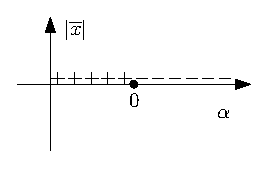
\includegraphics{3_1.eps}
\caption*{Бифуркационная диаграмма}
\end{figure}
\begin{flalign*}
& \underline{\alpha} > 0: \Omega = U_{\varepsilon \setminus \{0\}} &\\
& V(\v x) > 0, \quad \dot V(\v x) > 0, \quad \forall \v x \in \Omega &\\
& V(0) = 0, \quad V(\v x) = 0, \quad \forall \v x \in \partial \Omega (x = 0) &\\
& \Rightarrow \text{ неустойчивость, т.к. } \dot V = 0 \Rightarrow x = y = 0 &\\
\end{flalign*}
\end{xmp}

\begin{equation}
\label{threesta}
\det (A - \lambda E) = 0 \qquad a_0 \lambda^n + a_1\lambda^{n - 1} + \ldots + a_n = 0, \quad a_0 > 0
\end{equation}

\begin{xmp}
\begin{flalign*}
& n = 2: a_0\lambda^2 + a_1\lambda + a_2 = 0,\; a_0 > 0 &\\
& a_1^2 \geqslant 4a_0a_2 : \lambda_1 + \lambda_2 = - \frac{a_1}{a_0}, \; \lambda_1\lambda_2 = \frac{a_2}{a_0} &\\
& \re \lambda_{1, 2} = \lambda_{1, 2} < 0 \Leftrightarrow a_2 >0, a_1 > 0 &\\
& a_1^2 < 4a_0a_2: \re \lambda_{1, 2} = -\frac{a_1}{a_0} < 0 \Rightarrow a_2 >0, a_1 > 0 &\\
& \re \lambda_{1, 2} < 0 \Leftrightarrow a_i > 0, \; i = 1, 2 &\\
\end{flalign*}
\end{xmp}

\begin{ass}[Необходимое условие устойчивости]
Если все корни \eqref{threesta} при $n > 2$ имеют отрицательные вещественные части, то коэффициенты этого уравнения положительны:
\[
	\re \lambda_i < 0 \Rightarrow a_i > 0 \quad i = 1, \ldots, n
\]
\end{ass}
\begin{proof}
\begin{flalign*}
& \lambda_1, \ldots, \lambda_k \text{ --- действительные корни, } \lambda_i < 0,\; i = 1, \ldots, k &\\
& \lambda = \alpha_i \pm \beta_i i \quad j = 1, \ldots, m &\\
& f(\lambda) = a_0(\lambda - \lambda_1) \cdot \ldots \cdot (\lambda - \lambda_k)(\lambda - \alpha_1 - \beta_1 i) \cdot \ldots \cdot (\lambda - \alpha_1 + \beta_1 i)\cdot \ldots &\\ 
& = a_0(\lambda + \abs{\lambda_1}) \cdot \ldots \cdot (\lambda + \abs{\lambda_k})((\lambda + \abs{\alpha_1})^2 + \beta_1^2)\cdot \ldots = a_0\lambda^n + a_1\lambda^{n - 1} + \ldots + a_n \quad a_i > 0 \quad i = 1, \ldots, n &\\
\end{flalign*}
\end{proof}

\begin{xmp}
\[
	f(\lambda) = (\lambda^2 + 1)(\lambda + 1) = \lambda^3 + \lambda^2 + \lambda + 1 
\]
\end{xmp}

\begin{teo}[Критерий Рауса-Гурвица][б/д] 
$\forall i \re \lambda_i < 0 \Leftrightarrow$ все главные диагональные миноры определены положительно
\[
	\Delta = \left(
	\begin{matrix}
	a_1 & a_3 & a_5 & \ldots & 0 \\
	a_0 & a_2 & a_4 & \ldots & 0 \\
	0 & a_1 & a_3 & \ldots & 0 \\
	\vdots & & & \ddots & \vdots \\
	0 & 0 & 0 & \ldots & a_n \\
	\end{matrix}
	\right),
	\qquad \Delta_i > 0
\]
\end{teo}

\begin{ntc}
\[
	\Delta_n = a_n \Delta_{n - 1}
\]
\end{ntc}

\subsection{Равновесие натуральных систем}
Натуральная система:
\begin{gather*}
	L = \frac{1}{2}(A(\v q)\dv q, \dv q) - \Pi(\v q) \\
	\dv x = f(\v x), \; \v x = (q_1, \ldots, q_n, \dot q_1, \ldots, \dot q_n) \\
	\v q = \v q_0 \text{ --- равновесие}, \; \left(\left. \pd{\Pi}{q}\right|_{\v q = \v q_0} = 0 \right)
\end{gather*}
\begin{df}
$\v q = \v q_0$ --- установившееся равновесие положение равновесия натуральной системы, если
\[
	\forall \varepsilon > 0 \; \exists \delta > 0 \; \norm{\v q(0) - \v q_0} + \norm{\dv q(0)} < \delta \Rightarrow \norm{\v q(t) - \v q_0} + \norm{\dv q(t)} < \varepsilon \; \forall t > 0.
\]
\end{df}

\begin{teo}[Лагранжа-Дирихле]
Точка строго локального минимума потенциальной энергии натуральной системы является устойчивым по Ляпунову положением равновесия этой системы:
\end{teo}
\begin{proof}
\begin{flalign*}
& V = T + \Pi(\v q) - \Pi(\v q_0) &\\
& 1)\; V \vert_{\v q = \v q_0,\; \dv q = 0} = 0, V(\v q, \dv q) = \frac{1}{2}(A\dv q, \dv q) + \Pi(\v q) - \Pi(\v q_0) > 0 \quad (A \text { --- положительно определенная}) &\\
& \forall \v q, \dv q: \delta > \norm{\dv q} + \norm {\v q - \v q_0} > 0 &\\
& 2)\; \dot V = 0 \Rightarrow \dv q = 0, \v q = \v q_0 \text{ --- устойчиво.}
\end{flalign*}
\end{proof}

\begin{xmp}
\begin{flalign*}
& \Pi = \begin{cases}
0,\; q = 0 \\
e^{ -\frac{1}{\abs{q}}} \cdot \cos \frac{1}{\abs{q}},\; q \neq 0 
\end{cases} &\\
& 1)\; q = 0 \text{ --- положение равновесия} &\\
& 2)\; q = 0 \neq \min \Pi &\\
& 3)\; T + \Pi = h = const &\\
& \Pi \leqslant h, \; x = 0 \text{ --- устойчиво по Ляпунову (по опр.)} &\\
\end{flalign*}
\begin{figure}[H]
	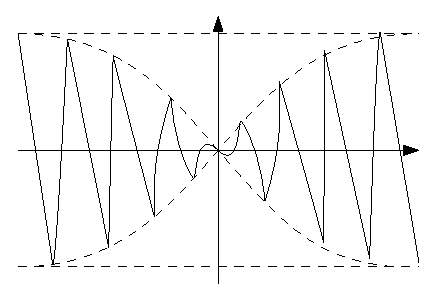
\includegraphics{3_2.eps}
\end{figure}
\end{xmp}
\begin{flalign*}
& \Pi(\v q) = \Pi(\v q_0) + \Pi^{(1)}(\v q) + \Pi^{(2)}(\v q) + \ldots + \Pi^{(m)}(\v q) &\\
& \Pi^{(1)} = \left.\pd{\Pi}{\v q}\right|_{\v q = \v q_0}(\v q - \v q_0) = 0 &\\
& \Pi^{(m)} \text{ --- первая нетривиальная форма } \Pi
\end{flalign*}
